\chapter{Aufgabe 6}
\section{Pointer}
\textit{Pointer} oder auch auf deutsch \textit{Zeiger}, sind eigene Datentypen in der Programmiersprache C.
Zeiger enthalten die Adressen von Speicherbereichen und bildet somit eine Brücke zur Hardware.
Durch diese ist ein direkter Zugriff auf diese Speicherbereiche möglich und somit auch das manipulieren der Daten in diesem Bereich.\par
Jeder Datentyp in C hat einen dazugehörigen Zeigertyp\cite{boekelmann:2023}.\par

\begin{lstlisting}
int a = 23 ;
int* zeiger_a = &a ;
float b = 53.42 ;
float* zeiger_b = &b ;
char c = 'z' ;
char* zeiger_c = &c ;
\end{lstlisting}

Wie in dem Beispiel zu sehen ist gibt es für jeden Datentyp einen dazugehörigen Zeigertyp.
Der Zeiger wird dabei mit dem \& Operator und dem Variablennamen initialisiert.
Er erhält somit den Speicherbereich in dem sich diese Variable befindet und nicht den direkten Wert den diese Variable besitzt.\par
Die Zeiger können auch Funktionen übergeben werden.
Somit wird beim Aufruf keine Kopie der Werte der Variablen erstellt, sonder die Funktion kann direkt mit den Speicherbereichen arbeiten und sich dort befindliche Werte manipulieren.
Im Falle eines Arrays muss hierfür nicht einmal ein extra Zeiger deklariert werden, da diese Standardmäßig als Zeiger an Funktionen übergeben werden.
Dies führt zu effizienteren Code und spart durch das wegfallen der Kopien Speicher ein.
Dies kann besonders wichtig auf \textit{freestanding} Implementierungen, wie Mikrocontroller, werden.\cite{boekelmann:2023}\par

\section{Pointerarithmetik}
Unter dem Begriff \textit{Pointerarithmetik} oder \textit{Zeigerarithmetik} versteht man das Addieren oder Subtrahieren auf Zeigerwerte.
Dies ermöglicht es auf Teile des Speichers zuzugreifen die in der Nähe des Zeigerwertes liegen.
Dies kann hilfreich dabei sein durch ein Array zu navigieren, da der Zeiger beim Initialisieren die Speicheradresse des ersten Wertes des Arrays erhält.
Um sich durch das Array zu bewegen wird also eine Veränderung des Zeigerwertes benötigt um die weiteren Speicherbereiche zu erreichen.\par
Allerdings muss dies mit Vorsicht behandelt werden.
Durch unvorsichtige Operationen kann unbeabsichtigt auf Speicherbereiche zugegriffen werden, die nicht für dieses Programm reserviert sind.
Dies kann zu Fehlern und Sicherheitsproblemen führen\cite{boekelmann:2023}.\par

\section{Repo}
In diesem Repo auf Gitlab befindet sich der Programmierteil der Aufgabe 6. In dieser Aufgabe sollte ein Beispiel Programm zum Umgang mit Zeigern erstellt werden. Dazu wird einmal ein integer mit Zeiger an eine Funktion übergeben, ein Zeiger auf ein Array und ein Zeiger auf ein struct an eine Funktion übergeben.\par
\href{https://gitlab.thga.de/daniel.krueger/pruefung_sose_2023_aufgabe_6_pointer}{\textbf{LINK}}

\section{Speicherdiagramm des Programms}
Die Abbildung \ref{speicherdiagramm} stellt die beispielhafte Speicherbelegung des C-Programms aus der Aufgabe 6 dar.\par

\begin{figure}[h]
	\centering
	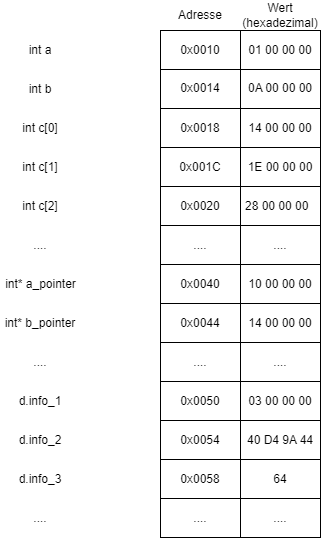
\includegraphics[scale=0.5]{Images/speicherdiagramm_aufgabe6.png}
	\caption{Beispiel der Speicherbelegung des Programms aus Aufgabe 6}
	\label{speicherdiagramm}
\end{figure}
